\documentclass[springer.tex]{subfiles}
\graphicspath{ {./figures/} }

\begin{document}

\abstract{
  Introductory text about the objectivs of this chapter
  \begin{itemize}
  \item \dots
  \end{itemize}
}

\chapter{Recursion}
\label{sec:recursion}
Recursion is a central concept in F\# and is used to control flow in loops without the \keyword{for} and \keyword{while} constructions. \Cref{fig:foreverRecursion} illustrates the concept of an infinite loop with recursion. 
\begin{figure} % We want the figure on the first page with the chapter title
  \centering
  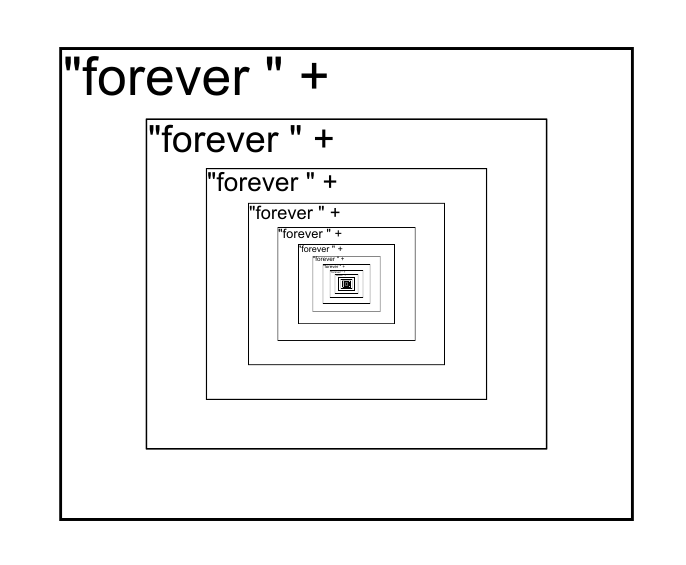
\includegraphics[width=0.6\textwidth]{recursion.png} % for some reason, it does not want to read the pdf-file
  \caption{An infinitely long string of "forever forever forever...", conceptually calculated by \mbox{\lstinline{let rec forever () = "forever " + (forever ()).}}}
  \label{fig:foreverRecursion}
\end{figure}

\section{Recursive Functions}
A \idx{recursive function} is a function which calls itself, and the syntax for defining recursive functions is an extension of that for regular functions:
%
\begin{verbatimwrite}{\ebnf/recursive.ebnf}
let rec <*ident*> = <*expr*> {*and <*ident*> = <*expr*>*} [*in*] <*expr*>
\end{verbatimwrite}
\syntax{\ebnf/recursive.ebnf}{Syntax for defining one or more mutually dependent recursive functions.}
%
From a compiler point of view, the \idx[rec@\lstinline{rec}]{\keyword{rec}} is necessary, since the function is used before the compiler has completed its analysis. If two functions are mutually recursive, then they must be defined jointly using the \idx[and@\lstinline{and}]{\keyword{and}} keyword.

An example of a recursive function that counts from 1 to 10 similarly to \Cref{count} is given in \Cref{countRecursive}.
%
\fs{countRecursive}{Counting to 10 using recursion.}
%
Here the \lstinline!prt! function calls itself repeatedly, such that the first call is \lstinline!prt 1 10!, which calls \lstinline!prt 2 10!, and so on until the last call \lstinline!prt 11 10!. Each time \lstinline{prt} is called, new bindings named \lstinline{a} and \lstinline{b} are made to new values. This is illustrated in \Cref{fig:countRecursiveScopes}.
\begin{figure} % make sure figure is printed after the countRecursive
  \begin{tcolorbox}[reset,valign lower=bottom,right=0.01\linewidth,squeezed title={\lstinline[language=console]{\$ fsharpc countRecursive.fsx \&\& mono countRecursive.exe}}]
    \lstinline{prt 1 10}
    \begin{tcbraster}[raster columns=1,raster equal height,raster halign=right]
      \begin{tcolorbox}[valign lower=bottom,right=0.01\linewidth,squeezed title={\lstinline{prt}$_1$: \lstinline{a}$_1$\lstinline{ = 1}, \lstinline{b}$_1$\lstinline{ = 10}}]
        \lstinline{1 > 10:} \xmark\\
        \hspace*{0.03\linewidth}\lstinline{printf "1 "}\\
        \hspace*{0.03\linewidth}\lstinline{prt 2 10}
        \begin{tcbraster}[raster width=0.97\linewidth]
          \begin{tcolorbox}[valign lower=bottom,right=0.01\linewidth,squeezed title={\lstinline{prt}$_2$: \lstinline{a}$_2$\lstinline{ = 2}, \lstinline{b}$_2$\lstinline{ = 10}}]
            \lstinline{2 > 10:} \xmark\\
            \hspace*{0.03\linewidth}\lstinline{printf "2 "}\\
            \hspace*{0.03\linewidth}\lstinline{prt 3 10}
            \begin{tcbraster}[raster width=0.97\linewidth]
              \begin{tcolorbox}[valign lower=bottom,right=0.01\linewidth,squeezed title={\lstinline{prt}$_3$: \lstinline{a}$_3$\lstinline{ = 3}, \lstinline{b}$_3$\lstinline{ = 10}}]
                \lstinline{3 > 10:} \xmark\\
                \hspace*{0.03\linewidth}\lstinline{printf "3 "}\\
                \hspace*{0.03\linewidth}\lstinline{prt 4 10}\\
                \hspace*{0.06\linewidth}$\ddots$\\
                \hspace*{0.09\linewidth}\lstinline{prt 11 10}
                \begin{tcbraster}[,raster width=0.91\linewidth]
                  \begin{tcolorbox}[valign lower=bottom,right=0.01\linewidth,squeezed title={\lstinline{prt}$_{11}$: \lstinline{a}$_{11}$\lstinline{ = 1}, \lstinline{b}$_{11}$\lstinline{ = 10}}]
                    \lstinline{11 > 10} \cmark\\
                    \hspace*{5mm}\lstinline{printf "\\n"}
                    \tcblower
                    \lstinline{()}
                  \end{tcolorbox}
                \end{tcbraster}
                \hspace*{0.06\linewidth}\reflectbox{$\ddots$}
                \tcblower
                \lstinline{()}
              \end{tcolorbox}
            \end{tcbraster}
            \tcblower
            \lstinline{()}
          \end{tcolorbox}
        \end{tcbraster}
        \tcblower
        \lstinline{()}
      \end{tcolorbox}
    \end{tcbraster}
    \tcblower
    \lstinline{()}
  \end{tcolorbox}
  \caption{Illustration of the recursion used to write the sequence ``1 2 3 ... 10'' in line~\ref{countRecursiveCall} in \Cref{countRecursive}. Each frame corresponds to a call to \lstinline{prt}, where new values overshadow old ones. All calls return \lstinline{unit}.}
  \label{fig:countRecursiveScopes}
\end{figure}
The old values are no longer accessible, as indicated by subscripts in the figure. E.g., in \lstinline{prt}$_3$, the scope has access to \lstinline{a}$_3$ but not \lstinline{a}$_2$ and \lstinline{a}$_1$. Thus, in this program, the process is similar to a \lstinline{for} loop, where the counter is \lstinline{a}, and in each loop its value is reduced.

The structure of the function is typical for recursive functions. They very often follow the following pattern.
\begin{verbatimwrite}{\ebnf/recursivePattern.ebnf}
let rec f a =
  §\tikzmark{recursivePatternCriteriumStart}§if <*stopping condition*>§\tikzmark{recursivePatternCriteriumStop}§
  then §\tikzmark{recursivePatternStopStart}§<*stopping step*>§\tikzmark{recursivePatternStopEnd}§
  else §\tikzmark{recursivePatternRecurseStart}§<*recursion step*>§\tikzmark{recursivePatternRecurseEnd}§
\end{verbatimwrite}
\syntax[]{\ebnf/recursivePattern.ebnf}{Recursive functions consist of a stopping criterium, a stopping expression, and a recursive step.}%
%\FrameArea{recursivePatternCriteriumStart}{recursivePatternCriteriumStop}%
%\FrameArea{recursivePatternStopStart}{recursivePatternStopEnd}%
%\FrameArea{recursivePatternRecurseStart}{recursivePatternRecurseEnd}%
The \idx[match@\lstinline{match}]{\keyword{match}} -- \idx[with@\lstinline{with}]{\keyword{with}} are also very common conditional structures. In \Cref{countRecursive}, \lstinline{a > b} is the \idx{stopping condition}, \lstinline{printfn "\n"} is the \idx{stopping step}, and \lstinline{printfn "\%d " a; prt (a + 1) b} is the \idx{recursion step}.


\begin{comment}
  The syntax for defining recursive functions in F\# is,
%
  \begin{verbatimwrite}{tmp.ebnf}
    expr = ...  | "let" "rec" functionDefn {"and" functionDefn} "in"
    expr
  \end{verbatimwrite}
  \ebnf{tmp.ebnf}{Recursive functions.}
%
\end{comment}
\afterpage{\clearpage} % flush floats

\section{The Call Stack and Tail Recursion}
\label{sec:callStack}
Fibonacci's sequence of numbers is a recursive sequence of numbers with relations to the Golden ratio and structures in biology. The Fibonacci sequence is the sequence of numbers $1, 1, 2, 3, 5, 8, 13, \ldots$. The sequence starts with $1, 1$ and the next number is recursively given as the sum of the two previous ones. A direct implementation of this is given in \Cref{fibFor}.
%
\fs{fibRecursive}{The $n$'th Fibonacci number using recursion.}
%
Here we extended the sequence to $0, 1, 1, 2, 3, 5, \ldots$ with the starting sequence $0, 1$, allowing us to define all $\text{fib}(n)=0,\, n < 1$. Thus, our function is defined for all integers, and for the irrelevant negative arguments it fails gracefully by returning 0. This is a general piece of advice: \advice{make functions that fail gracefully.} 
%The recursive definition allows for recursive value definitions and defining several values and functions in one expression. Recursive values are particularly useful for defining infinite sequences, see \Cref{sec:sequences}.

A visualization of the calls and the scopes created by \lstinline{fibRecursive} is shown in \Cref{fig:fibRecursiveScope}.
\begin{figure} % make sure figure is printed after the countRecursive
  \begin{tcolorbox}[reset,valign lower=bottom,right=0.01\linewidth,squeezed title={\lstinline[language=console]{\$ fsharpc fibRecursive.fsx \&\& mono fibRecursive.exe}}]%,squeezed title=\lstinline[language=console]{\$ fsharpc fibRecursive.fsx \&\& mono fibRecursive.exe}]
    \lstinline{fib 3}
    \begin{tcbraster}[raster columns=1,raster equal height,raster halign=right]
      \begin{tcolorbox}[valign lower=bottom,right=0.01\linewidth,squeezed title={\lstinline{fib}$_1$: \lstinline{n}$_1$\lstinline{ = 3}}]
        \lstinline{3 < 1:} \xmark\\
        \hspace*{0.03\linewidth}\lstinline{3 = 1:} \xmark\\
        \hspace*{0.06\linewidth}\lstinline{fib 2 + fib 1}
        \begin{tcbraster}[raster columns=2,raster width=0.94\linewidth]
          \begin{tcolorbox}[valign lower=bottom,right=0.01\linewidth,squeezed title={\lstinline{fib}$_2$: \lstinline{n}$_2$\lstinline{ = 2}}]
            \lstinline{2 < 1:} \xmark\\
            \hspace*{0.03\linewidth}\lstinline{2 = 1:} \xmark\\
            \hspace*{0.06\linewidth}\lstinline{fib 1 + fib 0}
            \begin{tcbraster}[raster columns=2,raster width=0.94\linewidth]
              \begin{tcolorbox}[valign lower=bottom,right=0.01\linewidth,squeezed title=\lstinline{fib}$_4$: \lstinline{n}$_4$\lstinline{ = 1}]
                \lstinline{1 < 1:} \xmark\\
                \hspace*{0.06\linewidth}\lstinline{1 = 1:} \cmark
                \tcblower
                \lstinline{1}
              \end{tcolorbox}
              \begin{tcolorbox}[valign lower=bottom,right=0.01\linewidth,squeezed title={\lstinline{fib}$_5$: \lstinline{n}$_5$\lstinline{ = 0}}]
                \lstinline{0 < 1:} \cmark
                \tcblower
                \lstinline{0}
              \end{tcolorbox}
            \end{tcbraster}
            \tcblower
            \lstinline{1}
          \end{tcolorbox}
          \begin{tcolorbox}[valign lower=bottom,right=0.01\linewidth,squeezed title={\lstinline{fib}$_3$: \lstinline{n}$_3$ \lstinline{ = 1}}]
            \lstinline{1 < 1:} \xmark\\
            \hspace*{0.03\linewidth}\lstinline{1 = 1:} \cmark
            \tcblower
            \lstinline{1}
          \end{tcolorbox}
        \end{tcbraster}
        \tcblower
        \lstinline{2}
      \end{tcolorbox}
    \end{tcbraster}
    \tcblower
    \lstinline{3}
  \end{tcolorbox}
  \caption{Illustration of the recursion used to write the sequence ``1 2 3 ... 10'' in line~\ref{countRecursiveCall} in \Cref{countRecursive}. Each frame corresponds to a call to \lstinline{fib}, where new values overshadow old ones.}
  \label{fig:fibRecursiveScope}
\end{figure}
The figure illustrates that each recursive step results in two calls to the function, thus creating two new scopes. And it gets worse. \Cref{fig:fibRecursiveScopeDeep} illustrates the tree of calls for \lstinline{fib 5}.
\begin{figure}
  \centering
  \Tree[.{\lstinline{fib 5}} 
             [.{\lstinline{fib 4}} 
               [.{\lstinline{fib 3}}
                 [.{\lstinline{fib 2}}
                   [.{\lstinline{fib 1}}
                   ]
                   [.{\lstinline{fib 0}}
                   ]
                 ]
                 [.{\lstinline{fib 1}}
                 ]
               ]
               [.{\lstinline{fib 2}}
                 [.{\lstinline{fib 1}}
                 ]
                 [.{\lstinline{fib 0}}
                 ]
               ]
             ]
             [.\lstinline{fib 3} 
               [.{\lstinline{fib 2}}
                 [.{\lstinline{fib 1}}
                 ]
                 [.{\lstinline{fib 0}}
                 ]
               ]
               [.{\lstinline{fib 1}}
               ]
             ]
           ]
  \caption{The function calls involved in calling \lstinline{fib 5}.}
  \label{fig:fibRecursiveScopeDeep}
\end{figure}
Thus, a call to the function \lstinline{fib} generates a tree of calls that is five levels deep and has \lstinline{fib(5)} number of nodes. In general for the program in \Cref{fibRecursive}, a call to \lstinline{fib(n)} produces a tree with $\text{\lstinline{fib(n)}}\leq c\alpha^n$ calls to the function for some positive constant $c$ and $\alpha \geq \frac{1+\sqrt{5}}{2}\sim 1.6$\jon{\url{https://math.stackexchange.com/questions/674533/prove-upper-bound-big-o-for-fibonaccis-sequence}}. Each call takes time and requires memory, and we have thus created a slow and somewhat memory-intensive function. This is a hugely ineffective implementation of calculating entries into Fibonacci's sequence, since many of the calls are identical. E.g., in \Cref{fig:fibRecursiveScopeDeep}, \lstinline{fib 1} is called five times. Before we examine a faster algorithm, we first need to discuss how F\# executes function calls.

When a function is called, then memory is dynamically allocated internally for the function on what is known as the \idx{call stack}. Stacks are used for many things in programming, but typically the call stack is considered special, since it is almost always implicitly part of any program execution. Hence, it is often just referred to as \idx{The Stack}. When a function is called, a new \idx{stack frame} is stacked (pushed) on the call stack, including its arguments, local storage such as mutable values, and where execution should return to when the function is finished. When the function finishes, the stack frame is unstacked (popped) and in its stead, the return value of the function is stacked. This return value is then unstacked and used by the caller. After unstacking the return value, the call stack is identical to its state prior to the call. \Cref{fig:TheStack} shows snapshots of the call stack when calling \lstinline{fib 5} in \Cref{fibRecursive}. 
\begin{figure}
  \centering
  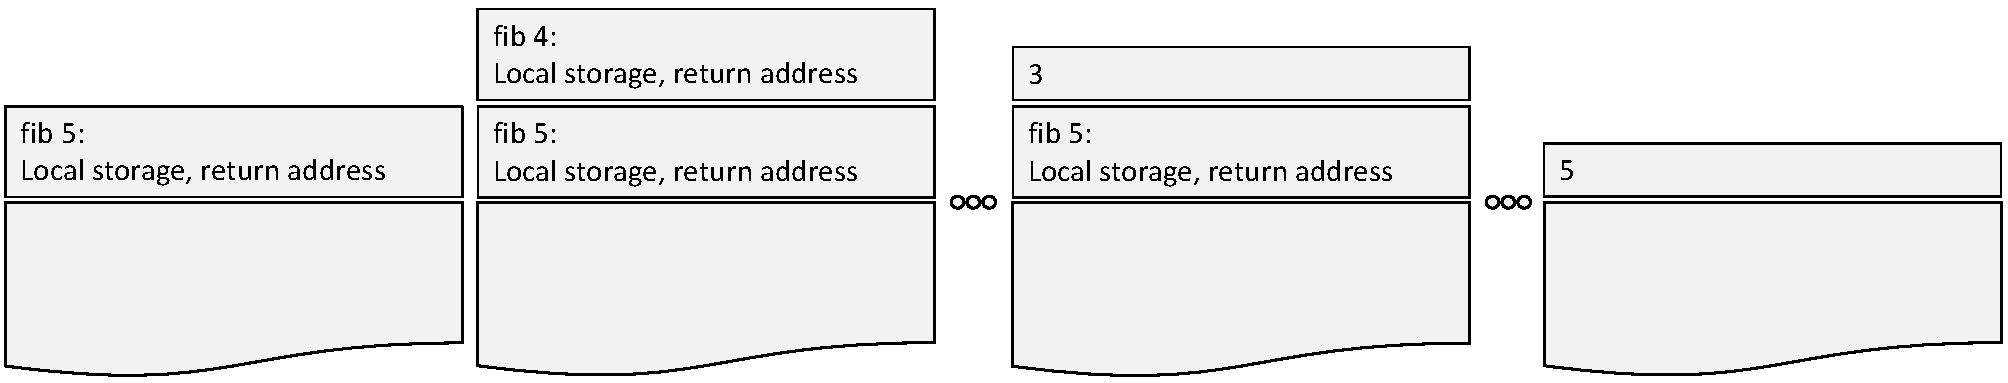
\includegraphics[width=\textwidth]{TheCallStack}
  \caption{A call to \lstinline{fib 5} in \Cref{fibRecursive} starts a sequence of function calls and stack frames on the call stack.}
  \label{fig:TheStack}
\end{figure}
The call first stacks a frame onto the call stack with everything needed to execute the function body plus a reference to where the return to, when the execution is finished. Then the body of \lstinline{fib} is executed, which includes calling \lstinline{fib 4} and \lstinline{fib 3} in turn. The call to \lstinline{fib 4} stacks a frame onto the call stack, and its body is executed. Once execution is returned from the call to \lstinline{fib 4}, the result of the function is on top of the stack. It is unstacked, saved and the call to \lstinline{fib 3} is treated equally. When the end of \lstinline{fib 5} is reached, its frame is unstacked, and its result is stacked. In this way, the call stack is returned to its original state except for the result of the function, and execution is returned to the point right after the original call to \lstinline{fib 5}. Thus, for \Cref{fibRecursive} $\mathcal{O}\left(\alpha^n\right),\; \alpha=\frac{1+\sqrt{5}}{2}$ stacking operations are performed for a call to \lstinline{fib n}. The $\mathcal{O}\left(f(n)\right)$ is the \idx{Landau symbol} used to denote the order of a function, such that if $g(n) = \mathcal{O}(f(n))$ then there exists two real numbers $M>0$ and a $n_0$ such that for all $n\geq n_0$, $|g(n)| \leq M |f(n)|$.\jon{Introduction of Landau notation needs to be moved earlier, since it used in Collections chapter.} As indicated by the tree in \Cref{fig:fibRecursiveScopeDeep}, the call tree is at most $n$ high, which corresponds to a maximum of $n$ additional stack frames as compared to the starting point.

The implementation of Fibonacci's sequence in \Cref{fibRecursive} can be improved to run faster and use less memory. One such algorithm is given in \Cref{fibRecursiveAlt}
%
\fs{fibRecursiveAlt}{A fast, recursive implementation of Fibonacci's numbers. Compare with \Cref{fibRecursive}.}
%
Calculating the 45th Fibonacci number a MacBook Pro, with a 2.9 GHz Intel Core i5 using \Cref{fibRecursive} takes about 11.2s while using \Cref{fibRecursiveAlt} is about 224 times faster and only takes 0.050s. The reason is that \lstinline{fib} in \Cref{fibRecursiveAlt} calculates every number in the sequence once and only once by processing the list recursively while maintaining the previous two values needed to calculate the next in the sequence. I.e., the function \lstinline{fibPair} transforms the pair \lstinline{(a,b)} to \lstinline{(b,a+b)} such that, e.g., the 4th and 5th pair \lstinline{(3,5)} is transformed into the 5th and the 6th pair \lstinline{(5,8)} in the sequence. What complicates the algorithm is that besides the transformation, we must keep track of when to stop, which here is done using a counter variable, that is recursively reduced by 1 until our stopping criterium.

\Cref{fibRecursiveAlt} also uses much less memory than \Cref{fibRecursive}, since its recursive call is the last expression in the function, and since the return value of two recursive calls to \lstinline{fibPair} is the same as the return value of the last. In fact, the return value of any number of recursive calls to \lstinline{fibPair} is the return value of the last. This structure is called \idx{tail-recursion}. Compilers can easily optimize the call stack usage for tail recursion, since when in this example \lstinline{fibPair} calls itself, then its frame is no longer needed, and may be replaced by the new \lstinline{fibPair} with the slight modification, that the return point should be to \lstinline{fib} and not the end of the previous \lstinline{fibPair}. Once the recursion reaches the stopping criteria, then instead of popping a long list of calls of \lstinline{fibPair} frames, then there is only one, and the return value is equal to the return value of the last call and the return point is to \lstinline{fib}. Thus, many stack frames in tail recursion are replaced by one. Hence, \advice{prefer tail-recursion whenever possible.}

\section{Mutually Recursive Functions}
Functions that recursively call each other are called \idx{mutually recursive} functions. F\# offers the \idx[let@\lstinline{let}]{\keyword{let}} -- \idx[rec@\lstinline{rec}]{\keyword{rec}} -- \idx[and@\lstinline{and}]{\keyword{and}} notation for co-defining mutually recursive functions. As an example, consider the function \mbox{\lstinline!even : int -> bool!}, which returns true if its argument is even and false otherwise, and the opposite function \mbox{\lstinline!odd : int -> bool!}. A mutually recursive implementation of these functions can be developed from the following relations: \mbox{\lstinline!even 0 = true!}, \mbox{\lstinline!odd 0 = false!}, and for $n>0$, \mbox{\lstinline!even n = odd (n-1)!}, which implies that for $n>0$, \mbox{\lstinline!odd n = even (n-1)!}:
%
\fs{mutuallyRecursive}{Using mutual recursion to implement even and odd functions.}
%
Notice that in the lightweight notation the \keyword{and} must be on the same indentation level as the original \keyword{let}.

Without the \keyword{and} keyword, F\# will issue a compile error at the definition of \lstinline!even!. However, it is possible to implement mutual recursion by using functions as an argument, e.g.,
%
\fs{mutuallyRecursiveAlt}{Mutual recursion without the \keyword{and} keyword requires a helper function.}
%
This being said, \Cref{mutuallyRecursive} is clearly to be preferred over \Cref{mutuallyRecursiveAlt}. 

In the example above, we used the \lstinline!even! and \lstinline!odd! function problems to demonstrate mutual recursion. There is, of course, a much simpler solution, which does not use recursion at all:
%
\fsCode{parity}{parity}{A better way to test for parity without recursion.}{}
%
This is to be preferred anytime as the solution to the problem. \jon{Here it would be nice to have an intermezzo, giving examples of how to write a recursive program by thinking the problem has been solved.}
\clearpage

\section{Tracing Recursive Programs}
\label{sec:recursiveTracing}
Tracing by hand is a very illustrative method for understanding recursive programs. Consider the recursive program in \Cref{gcd}.
%
\fs{gcd}{The greatest common divisor of 2 integers.}
%
The program includes a function for calculating the greatest common divisor of 2 integers, and calls this function with the numbers 10 and 15. Following the notation introduced in \Cref{sec:tracing}, we write:
\begin{quote}
  \begin{tabular*}{0.6\linewidth}{l|lll}
    Step & Line & Env.\ & Bindings and evaluations\\
    \hline
    0 & - & $E_0$ & ()\\
    1 &\ref{gcd:gcd} & $E_0$ & $\text{gcd} = \big((a, b), \text{gcd-body}, ()\big)$\\
    2 &\ref{gcd:a} & $E_0$ & $a = 10$\\
    3 &\ref{gcd:b} & $E_0$ & $b = 15$\\
  \end{tabular*}
\end{quote}
In line~\ref{gcd:printfn}, \lstinline!gdc! is called before any output is generated, which initiates a new environment $E_1$ and executes the code in gcd-body:
\begin{quote}
  \begin{tabular*}{0.6\linewidth}{l|lll}
    Step & Line & Env.\ & Bindings and evaluations\\
    \hline
  4 & \ref{gcd:printfn} & $E_0$ & $\text{gcd a b} = \text{?}$\\
  5 & \ref{gcd:gcd} & $E_1$ & $\big((a = 10, b =15), \text{gcd-body}, ()\big)$\\
  \end{tabular*}
\end{quote}
 In $E_1$ we have that $a<b$, which fulfills the first condition in line~\ref{gcd:if}. Hence, we call gdc with switched arguments and once again initiate a new environment,
\begin{quote}
  \begin{tabular*}{0.6\linewidth}{l|lll}
    Step & Line & Env.\ & Bindings and evaluations\\
    \hline
  6&\ref{gcd:gcdR1} & $E_1$ &$\text{gcd b a} = \text{?}$\\
  7 &\ref{gcd:gcd} & $E_2$ & $\big((a = 15, b = 10), \text{gcd-body}, ()\big)$\\
  \end{tabular*}
\end{quote}
In $E_2$, \lstinline!a < b! in line~\ref{gcd:if} is false, but
\lstinline!b > 0! in line~\ref{gcd:elif} is true, hence, we first
evaluate \lstinline{a % b}, call \lstinline{gcd b (a % b)}, and then create a new environment,
\begin{quote}
  \begin{tabular*}{0.6\linewidth}{l|lll}
    Step & Line & Env.\ & Bindings and evaluations\\
    \hline
    8&\ref{gcd:gcdR2} & $E_2$ & $\text{a \% b} = 5$\\
    9&\ref{gcd:gcdR2} & $E_2$ & $\text{gcd b (a \% b)} = \text{?}$\\
    10&\ref{gcd:gcd} & $E_3$ &$\big((a = 10, b = 5), \text{gcd-body}, ()\big)$\\
  \end{tabular*}
\end{quote}
Again we fall through to line~\ref{gcd:gcdR2}, evaluate the remainder operator and initiate a new environment,
\begin{quote}
  \begin{tabular*}{0.6\linewidth}{l|lll}
    Step & Line & Env.\ & Bindings and evaluations\\
    \hline
    11&\ref{gcd:gcdR2} & $E_3$ & $\text{a \% b} = 0$\\
    12&\ref{gcd:gcdR2} & $E_3$ & $\text{gcd b (a \% b)} = \text{?}$\\
    13&\ref{gcd:gcd} & $E_4$ & $\big((a = 5, b = 0), \text{gcd-body}, ()\big)$\\
  \end{tabular*}
\end{quote}
This time both \lstinline!a < b! and \lstinline!b > 0! are false, so we fall through to line~\ref{gcd:return} and return the value of \lstinline!a! from $E_4$, which is \lstinline!5!:
\begin{quote}
  \begin{tabular*}{0.6\linewidth}{l|lll}
    Step & Line & Env.\ & Bindings and evaluations\\
    \hline
    14&\ref{gcd:return} & $E_4$ & $\text{return} = 5$\\
  \end{tabular*}
\end{quote}
We scratch $E_4$, return to $E_3$, either physically or mentally replace the ?-mark with \lstinline!5! and continue the evaluation of line~\ref{gcd:gcdR2}. Since this is also a branch of the last statement in \lstinline{gdc}, we return the previously evaluated value,
\begin{quote}
  \begin{tabular*}{0.6\linewidth}{l|lll}
    Step & Line & Env.\ & Bindings and evaluations\\
    \hline
    15&\ref{gcd:gcdR2} & $E_3$ & $\text{return} = 5$\\
  \end{tabular*}
\end{quote}
Like before, we scratch $E_3$, return to $E_2$, either physically or mentally replace the ?-mark with \lstinline!5! and continue the evaluation of line~\ref{gcd:gcdR2}. Since this is also a branch of the last statement in \lstinline{gdc}, we return the just evaluated value,
\begin{quote}
  \begin{tabular*}{0.6\linewidth}{l|lll}
    Step & Line & Env.\ & Bindings and evaluations\\
    \hline
    16&\ref{gcd:gcdR2} & $E_2$ & $\text{return} = 5$\\
  \end{tabular*}
\end{quote}
Again, we scratch $E_2$, return to $E_1$, either physically or mentally replace the ?-mark with \lstinline!5! and continue the evaluation of line~\ref{gcd:gcdR2}. Since this is also a branch of the last statement in \lstinline{gdc}, we return the just evaluated value,
\begin{quote}
  \begin{tabular*}{0.6\linewidth}{l|lll}
    Step & Line & Env.\ & Bindings and evaluations\\
    \hline
    17&\ref{gcd:gcdR1} & $E_1$ & $\text{return} = 5$\\
  \end{tabular*}
\end{quote}
Finally, we scratch $E_1$, return to $E_0$, either physically or mentally replace the ?-mark with \lstinline!5! and continue the evaluation of line~\ref{gcd:gcdR2}:
\begin{quote}
  \begin{tabular*}{0.6\linewidth}{l|lll}3
    Step & Line & Env.\ & Bindings and evaluations\\
    \hline
    18 & \ref{gcd:printfn} & $E_0$ & $\text{output = "gcd a b = 5"}$\\
    19 & \ref{gcd:printfn} & $E_0$ & $\text{return = ()}$\\
  \end{tabular*}
\end{quote}
Note that the output of \lstinline{printfn} is a side-effect while its return-value is unit. In any case, since this is the last line in our program, we are done tracing.

\section{Key concepts and terms in this chapter}
Summary text about the key concepts from this chapter
\begin{itemize}
\item \ldots
\end{itemize}
\end{document}
